\documentclass[aspectratio=169]{beamer} %format: 16:9


% Alternatively, select ngerman
\usepackage[american]{babel}
%\usepackage[ngerman]{babel}

% For beginners: themes need to be in the same directory as this tex-file. For experts: no explanation required. ;)
\usetheme{ITD1}
% Choose whether you want the logo on each frame title. Can be changed at any
% time. Note: It adds some vertical white space to the frame's content pane.
\withoutframelogo
%\withoutframelogo

\usepackage{csquotes}
\usepackage{derivative}
\usepackage[
  backend=biber,
  doi=true,
  eprint=false,
  date=iso,
  seconds=true,
  style=alphabetic-verb,
  locallabelwidth=true,
  maxnames = 99,
  %citestyle=alphabetic-verb
  ]{biblatex}
\renewcommand*{\bibfont}{\footnotesize}

\addbibresource{literature.bib}
%\addbibresource{jrcisia-related.bib}

%\addglobalbib{strings-short.bib}
%\addbibresource[label=jrcisia-published]{jrcisia-published.bib}



\title{An Experimental Analysis of the Influence of the Precision of Parameters in an Artificial Neural Network}
% Uncomment if unwanted
\subtitle{Natural Computation PS Presentation 01}

% \author[J. Doe, J. Doe]{Jane Doe, John Doe}
\author[D. K., E. R., S. A. S., L. S.]{Denise Katritschenko, Elias Reich, Sayed Abozar Sadat, Lukas Schwaiger}
% \institute[\isiashort, \fhshort]{\isialong\\ \depitlong\\ \fhlong}
% \institute[\fhshort]{\isialong\\ \depitlong\\ \fhlong}
\institute[\plusshort]{\pluslong\\ Department of Artificial Intelligence and Human Interfaces (AIHI)}
\date[\today]{\today}


% Automatically add fullframe for section headers. Uncomment if you do not want
% them.
\AtBeginSection[]{\fullframe{\insertsectionhead}}

\begin{document}

\frame{\titlepage}


% \section{Introduction}

% below the presentation content starts
\begin{frame}{Primer on Neural Networks}
  \begin{figure}
    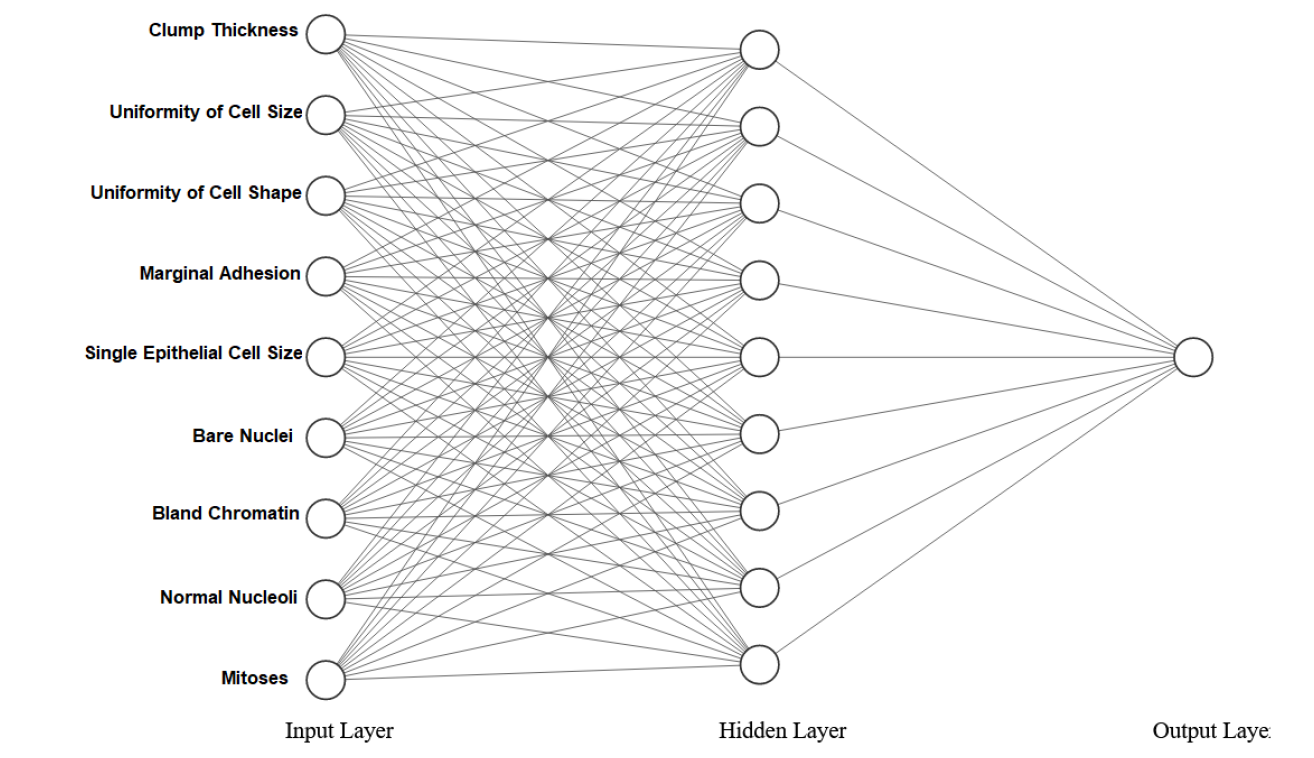
\includegraphics[width=0.9\textwidth]{figures/mlp.png}
  \end{figure}
\end{frame}

\begin{frame}{Single neuron view}
  \begin{figure}
    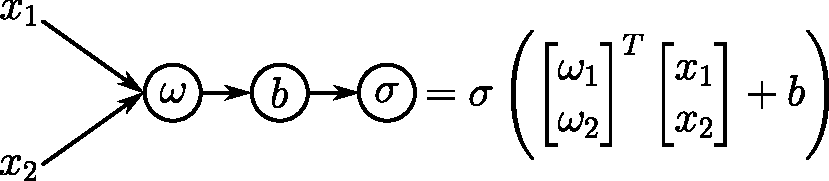
\includegraphics[width=0.96\textwidth]{figures/single-neuron.pdf}
  \end{figure}
\end{frame}

\begin{frame}{Gradients}
  \begin{itemize}
    \item Want to optimize the parameters $\omega$ and $b$.
    \item Need a target $y$ and error metric (loss $L$) to judge the networks predictions $\hat y$.
    \item Convex optimization is used to adjust the parameters.
    \item Many intermediate results need to be stored for efficient gradient computation.
  \end{itemize}

  \begin{align*}
    L(f(x_1, x_2)) &= (\sigma(\omega^T x + b) - y) ^2\\
                   &= (\sigma(a) - y) ^ 2\\
                   &= (\hat y - y) ^ 2
  \end{align*}
  \begin{alignat*}{3}
    \pdv{L}{\omega_1} &= \pdv{L}{\sigma} &&\pdv{\sigma}{a}      &&\pdv{a}{\omega_1}\\
                      &= 2(\hat y - y)~~ &&\odv{}{a}\sigma(a)~~ &&x_1
  \end{alignat*}
  
\end{frame}

\begin{frame}{Memory requirements}
  For NN training we need to store the following in memory:
  \begin{itemize}
    \item Inputs and output targets (possibly batched)
    \item Parameters (weights, biases, batch statistics, ...)
    \item Intermediate results
    \item Loss
    \item Gradients
  \end{itemize}

  For inference we only need the parameters.
  
\end{frame}

\begin{frame}{Example}
  \begin{figure}
    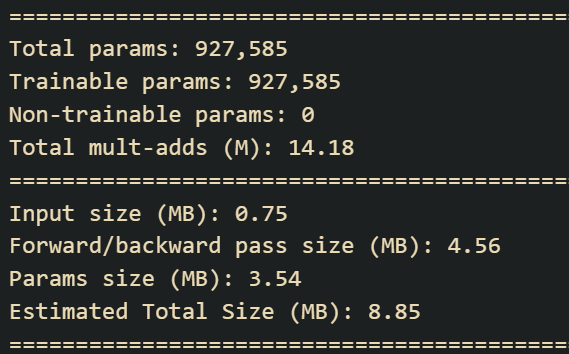
\includegraphics[width=0.8\textwidth]{figures/mobilenet-size.png}
  \end{figure}
\end{frame}

\begin{frame}{Reducing memory requirements}
  Without sacrificing precision one could reduce:
  \begin{itemize}
    \item Neurons per layer
    \item Number of layers
    \item Batch size
  \end{itemize}
  Naive downsizing can quickly lead to worse generalization and expressiveness or accuracy.\\

  $\rightarrow$ Keep the number of layers and parameters and only change the
  'bitwidth' of the parameters.
\end{frame}

\begin{frame}{How parameters are represented in memory}
\centering
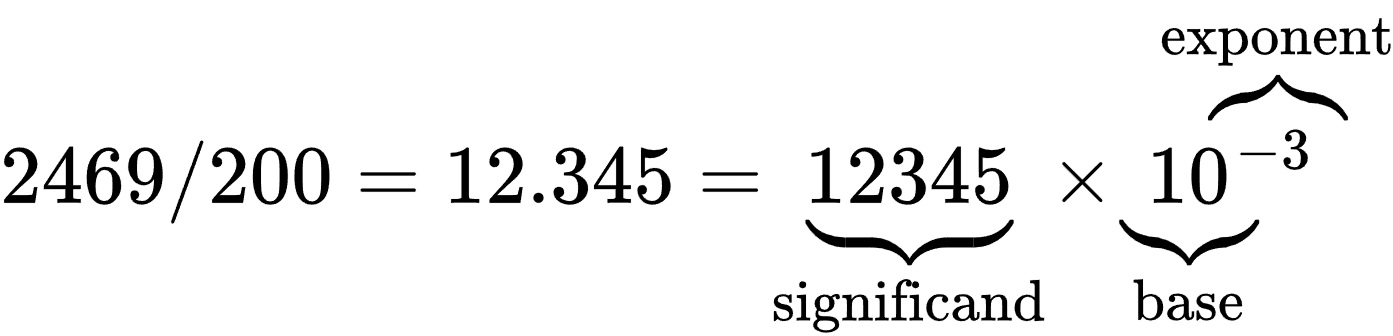
\includegraphics[width=0.8\textwidth]{figures/float.png}
\centering
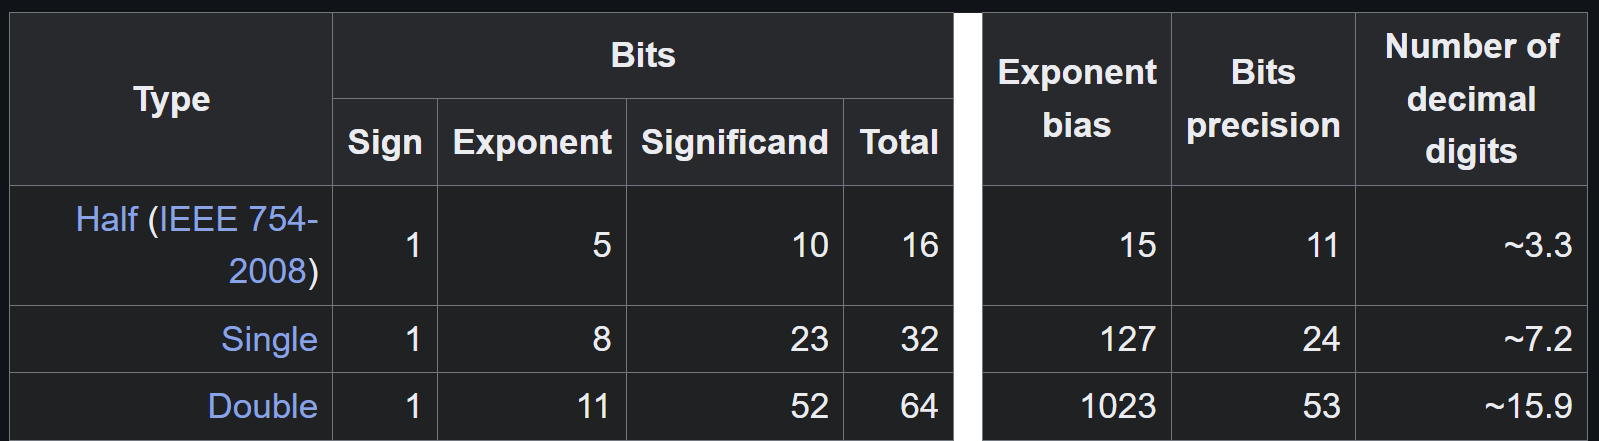
\includegraphics[width=0.8\textwidth]{figures/binary-formats.png}
\end{frame}

\begin{frame}{Related Work}
  \begin{enumerate}
    \item Training time precision reduction\begin{itemize}
      \item Mixed Precision Training. \emph{P. Micikevicius, 2017}
      \item Training Deep Neural Network in Limited Precision. \emph{H. Park, 2018}
      \item Dorefa-Net: Training Low Bitwidth Convolutional Neural Networks with low Bitwidth Gradients. \emph{S. Zhou, 2018}
      \item Training Deep Neural Networks with 8-bit Floating Point Numbers. \emph{N. Wang, 2018}
      \item Q-BERT: Hessian-Based Ultra Low-Precision Quantization of BERT. \emph{S. Shen, 2020}


    \end{itemize}
    \item Post training precision reduction\begin{itemize}
      \item Quantization and Training of Neural Networks for Efficient Integer-Arithmetic-Only Inference. \emph{J. Benoit, 2018}
      \item GPTQ: Accurate Post-Training Quantization for Generative Pre-trained Transformers. \emph{E. Frantar, 2022}
      \item SmoothQuant: Accurate and Efficient Post-Training Quantization for Large Language Models. \emph{G. Xiao, 2024}
    \end{itemize}
  \end{enumerate}

  There are also hardware specific optimizations, e.g. FPGA \emph{P. Vera 2020}, and many more.
\end{frame}

\begin{frame}{Results from literature}
  \begin{figure}
    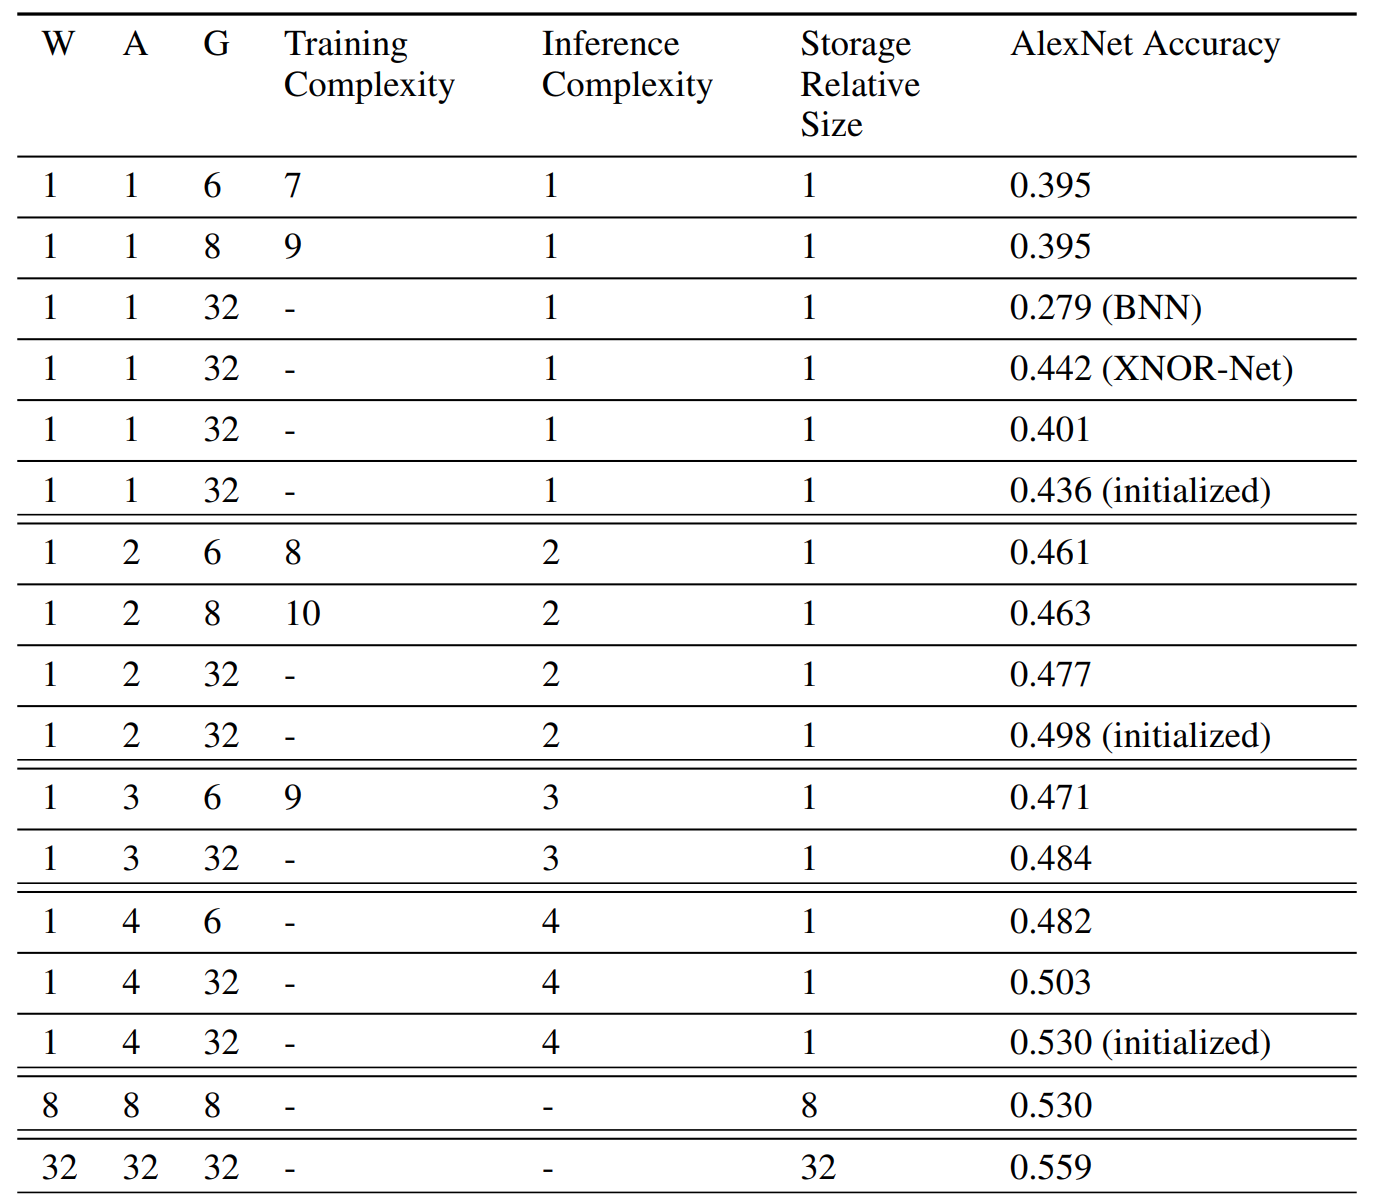
\includegraphics[width=0.5\textwidth]{figures/results-table.png}
    \caption{S. Zhou, 2018}
  \end{figure}
\end{frame}



\end{document}
